\chapter{GPS Variation Estimation}
\label{cha:GPS-variation-estimation}

The main component of the dataset is the GPS positional update events from the vehicles.
They contribute to 95\% of the events in the data, as shown by Figure \ref{fig:types-barplot} in Section \ref{sec:data-structure}.
An interesting high-level problem is thus the estimation of the variance in the GPS positions.
Manual inspection shows that the quality varies between trajectories and for different parts of the road network.
The quality also seems to change over time.
If there is a measurement for the variation in variance, one could make more informed decisions regarding the detection of bus stops and the determination of bus positions. 

The hypotheses are that the GPS positions vary depending on:
\begin{enumerate}
    \item \textit{Environment (Spatial Locality):} 
    The surrounding environment impacts the visibility of GPS satellites.
    For example, in an environment with a lot of reflections and obstacles, the precision of the GPS position will decrease.
    On the other hand, in open fields the precision will increase, as there are fewer obstacles blocking the GPS satellite signals.
    The environment can vary between different road segments, but also inside one road segment, e.g., a road can be partly covered by houses or trees.
    The variance can either be seen as continuous, where each point on the journey has its own variance, or as road segments, where each road segment has its own variance.
    In the continuous case, neighbouring pairs of points are connected and thus exhibit more similar variance, depending on the distance between the points (granularity) in a journey.
    In the case of road segments, different segments exhibit a potentially larger difference in variance.
    
    Road segments can either be created geographically, e.g., a segment is the road between two bus stops or between crossings, or contextually from the output of the continuous case.
    A geographical road segmentation most likely results in a higher average variance, as the environment potentially changes within the segment.
    The contextual segmentation can look at sequences of points in the journey, and group the sequential points which exhibit similar variance.
    The result is potentially segments where the inherent variance of each segment is lower than between different segments.

    Figure \ref{fig:gps-variation} illustrates how the GPS variance can differ for different road segments.
    In the shown scenario, the difference between geographical segmentation between crossings and contextual segmentation would be minor, as the variance seems to be similar for a given road segment.
    However, the difference is large if the geographical segmentation is done between bus stops.
    The number of road segments is higher in the crossing-geographical approach than in the contextual approach, as, for example, "Järnvägsgatan" has many crossings but exhibit similar variance. 
    
    \item \textit{GPS Sensor Calibration:}
    Each bus has its own GPS sensor, where different buses can have different sensor models with their own calibrations.
    In the general case the different GPS sensors show small variance due to different calibrations, environments, and satellite positions.
    However, occasionally they can vary, e.g., by some constant factor, as shown in Figure \ref{fig:gps-sensor-calibration}.
    The single orange-coloured bus journey seems to have a constant offset compared to the rest of the journeys for that particular bus line.
    The shown scenario is quite extreme, as the offset is large enough to cause problems with the Bus Stop Detection Algorithm in the IA component.
    No bus stops are detected in this particular scenario.
    The extreme situations can thus be detected by combining the positional event data with the bus stop event data.
    However, differences in calibrations which yield smaller offsets cannot be detected with this combining approach and are thus latent in the GPS variation estimation model.

    \item \textit{Time:}
    The timestamps of the position events affect the precision of the GPS sensor.
    At a single given point of the journey the precision could vary depending on the positions of satellites and the amount of satellites visible.
    The hypothesis is that there is a constant bias to the GPS positions depending on the time.
    The positions of the satellites thus cause a small offset to occur in the GPS position.
    This parameter probably has some periodicity, which could be fitted using a Gaussian Process with a periodical kernel.
    
\end{enumerate} 


\begin{figure}[ht!]
    \centering
    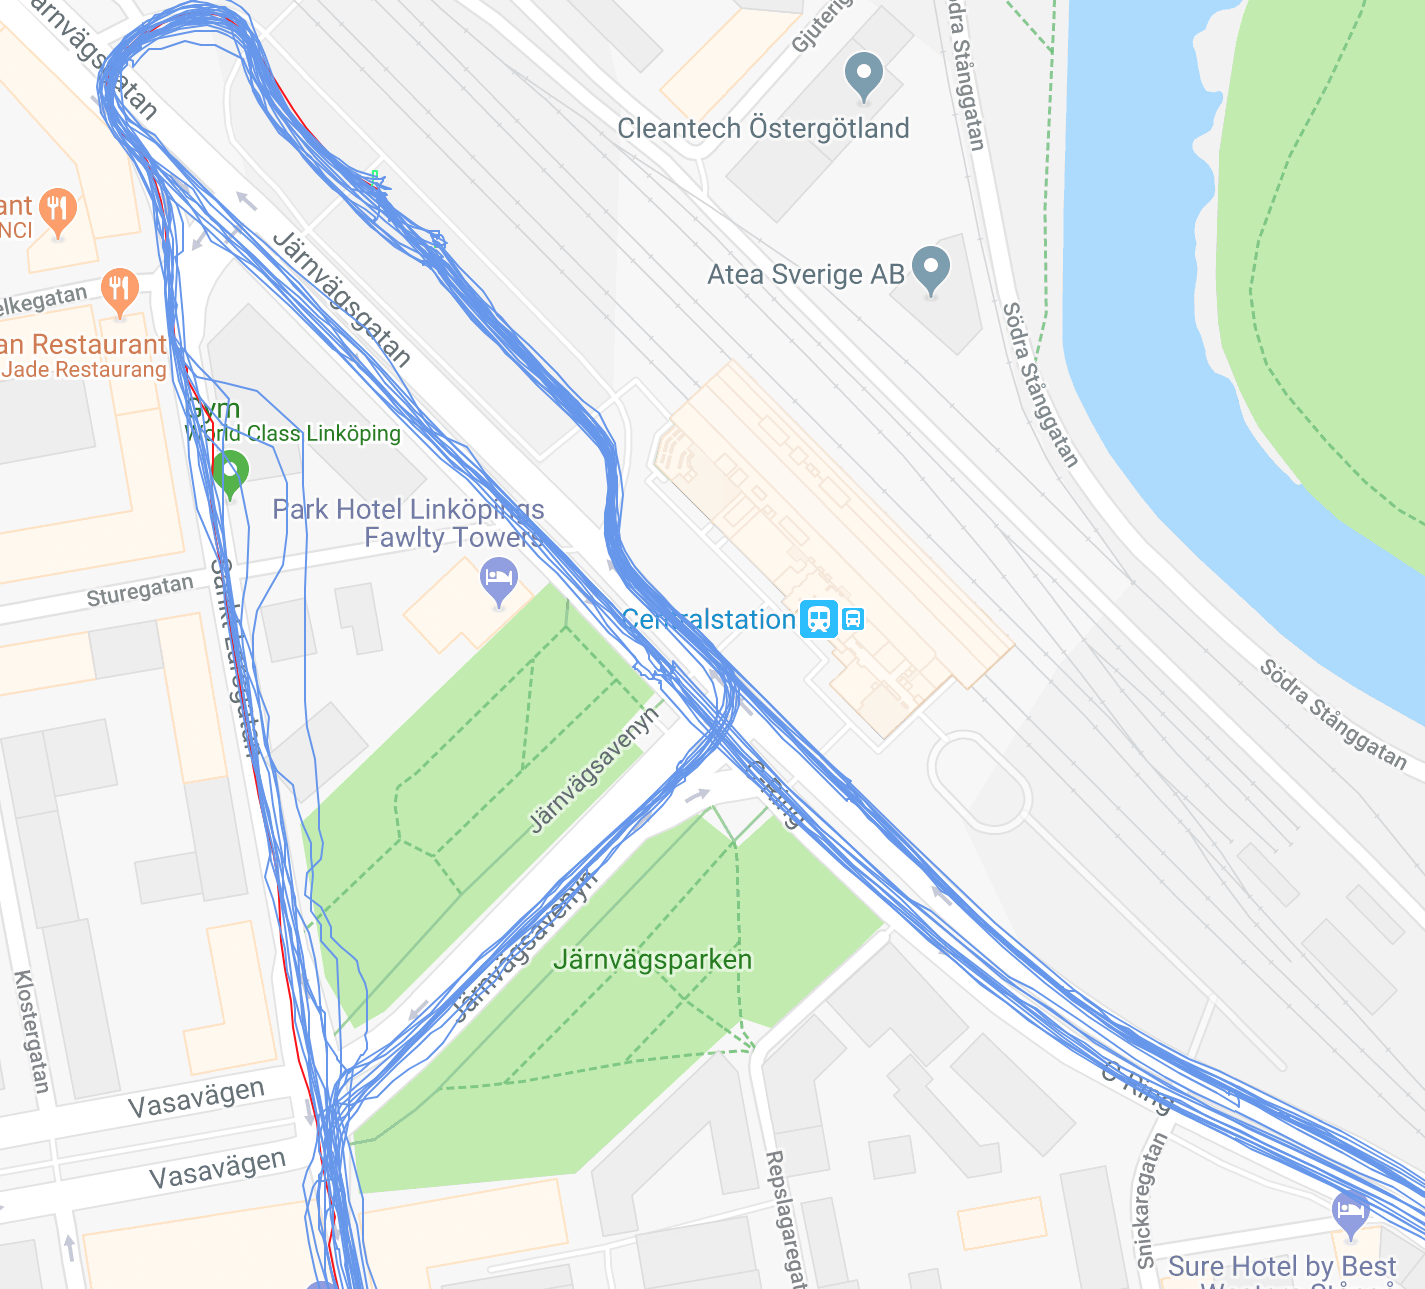
\includegraphics[width=0.7\textwidth]{figures/gps_variation}
    \caption[Visualisation of multiple journeys by different buses in the same area]
    {\small Visualisation of multiple journeys by different buses in the same area.
    Each blue line is a journey in the "Started" state.
    The variance differs between different road segments, as shown around "World Class Linköping" compared to "Järnvägsgatan".}
    \label{fig:gps-variation}
\end{figure}

\begin{figure}[ht!]
    \centering
    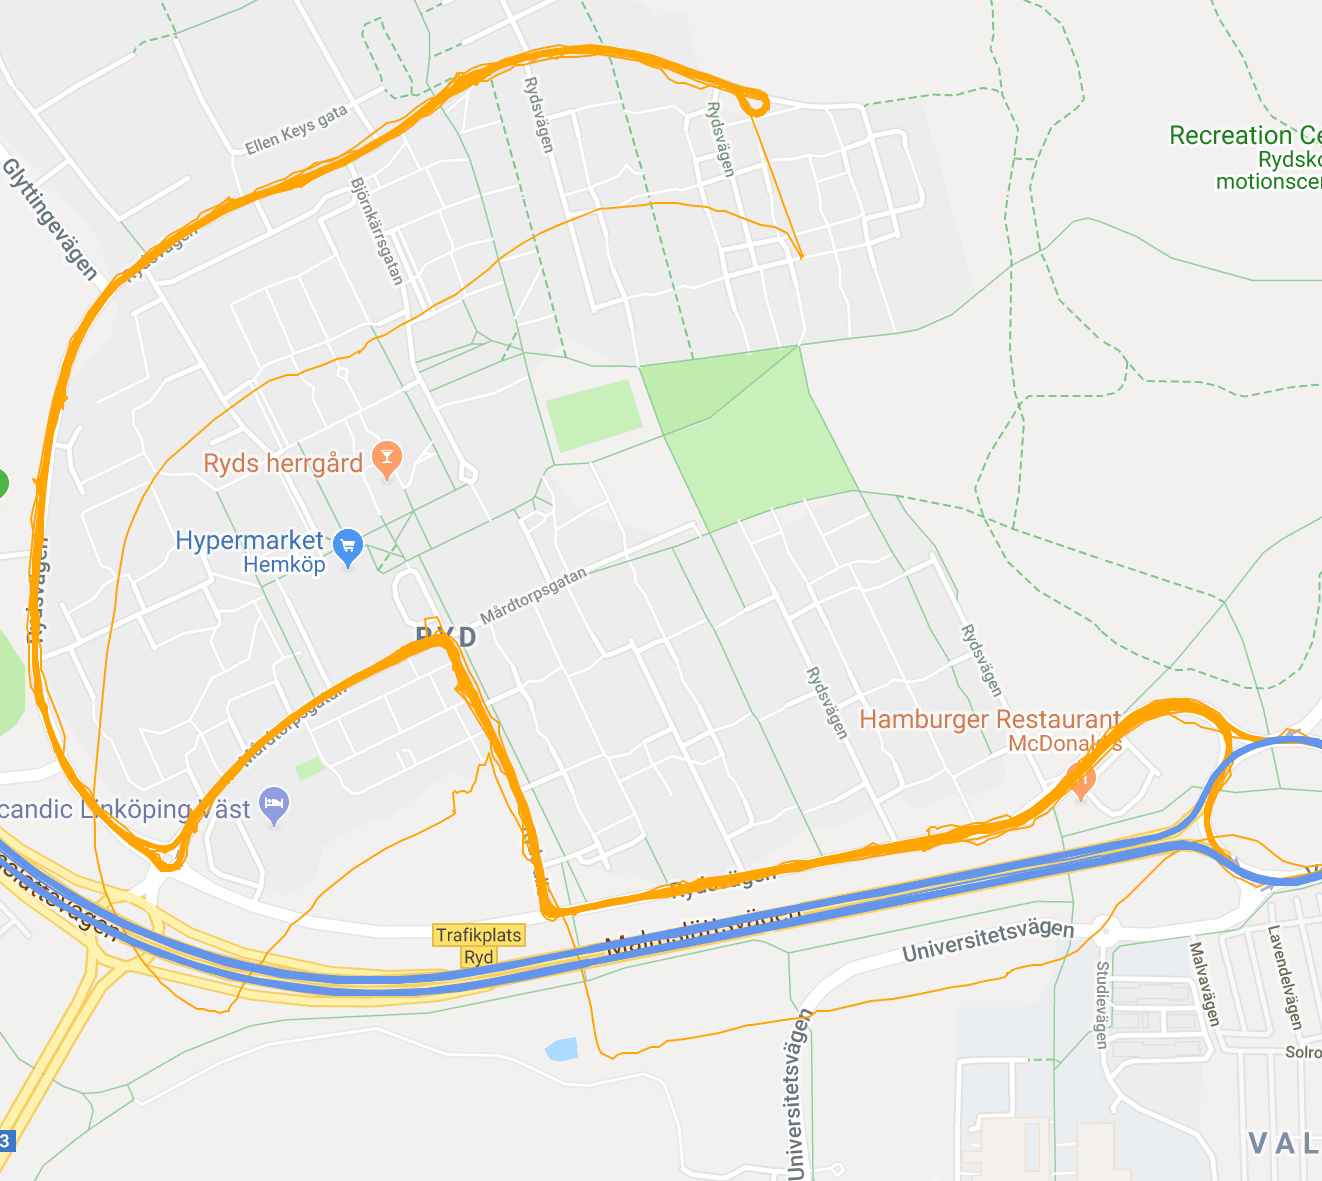
\includegraphics[width=0.7\textwidth]{figures/gps_sensor_calibration}
    \caption[Illustrates the case of a poorly calibrated GPS sensor on an individual bus]
    {\small Illustrates the case of a poorly calibrated GPS sensor on an individual bus.
    The orange lines creating the thicker line are all the other journeys for the same bus line, but done by other buses.
    The thin orange line is one bus with an extremely poorly calibrated GPS sensor.
    It seems to have a constant offset compared to the rest.
    This real-world scenario shows that the calibration of GPS sensors is important in order to produce useful data.}
    \label{fig:gps-sensor-calibration}
\end{figure}

In this thesis project, 37 trajectories from a single day is used.
Sections \ref{sec:stop-compression}-\ref{sec:probability-models} cover the methodology used for the GPS variation estimation.
The results are presented in Section \ref{sec:gps-var-result} and discussed in Section \ref{sec:gps-var-discussion}.  

\section{Stop Compression} \label{sec:stop-compression}
Each stop present in the journey causes an imbalance of points being clustered around that stop.
The longer the stop is, the more points are present.
This results in problems when using a GP model, as certain coordinates would thus be denser than others.
The GP would model the noise of the GPS in these denser areas, instead of the variance due to the environment.

Stop compression can be achieved in multiple ways, e.g., stopped positions could be either averaged or ignore completely.
The time of the stop is also adjusted.
In this thesis project, all \texttt{ObservedPositionEvent}s with a \textit{Speed} value lower than $0.1$ m/s are discarded and the time adjusted.
The result is a journey (trajectory) consisting of a sequence of coordinates where stops are invisible time-wise.

Examples of the procedure are shown in Figures \ref{fig:uncompressed-events} and \ref{fig:time-and-speed}.
Both figures show the same trajectory.
Figure \ref{fig:uncompressed-events} shows the trajectory without stop compression, where the stops are highlighted by drawn lines.
Figure \ref{fig:time-and-speed} shows the stop compressed speeds and coordinates of the trajectory.
The stop compression is implemented using a \textit{Speed} threshold value of $0.1$ m/s.

\begin{figure}[h!]
    \centering
    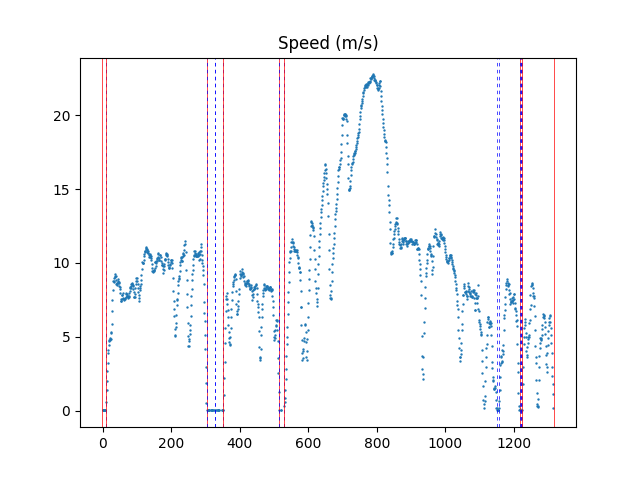
\includegraphics[width=0.9\textwidth]{figures/speed_and_stops_filter_0}
    \caption[Example of a trajectory with uncompressed speeds]
    {\small Example of a trajectory with uncompressed speeds.
    The red lines are \texttt{ArrivedEvent}s and \texttt{DepartedEvent}s.
    The dashed blue lines are \texttt{StartedEvent}s and \texttt{StoppedEvent}s.
    The red and blue lines usually coincide.}
    \label{fig:uncompressed-events}
\end{figure}

\begin{figure}[h!]
    \centering
    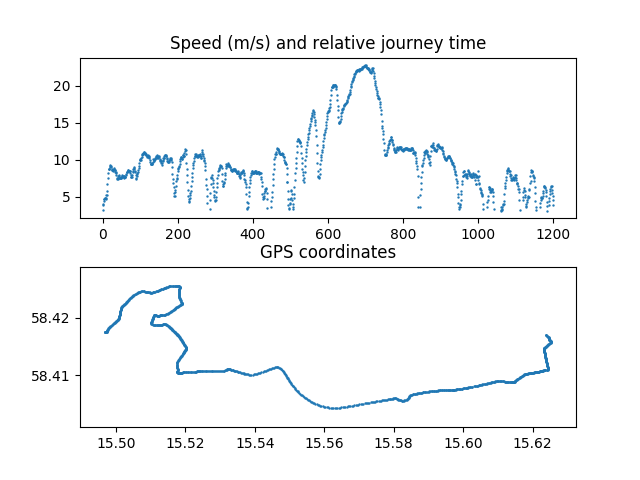
\includegraphics[width=0.9\textwidth]{figures/time_and_speed}
    \caption[Example of a stop compressed trajectory]
    {\small Example of a stop compressed trajectory.
    The \textit{Speed} threshold is set to $0.1$ m/s.
    The various speeds are shown in the top graph, while the trajectory is drawn in the bottom graph.}
    \label{fig:time-and-speed}
\end{figure}

\section{Synchronising Input Space} \label{sec:synchronisation}
Before GPs can be trained on the journey data, the journeys need to be synchronised in their input space.
A journey can be seen as a sequence of (longitude, latitude, time)-tuples, where \textit{time} is the timestamp of the bus when it is at coordinate (longitude, latitude).
However, at identical values for the \textit{time} parameter, different buses driving for the same bus line have progressed differently on the journey.
For example, buses drive at different speeds and they may stay stopped for different periods of time at each bus stop.
The \textit{time} parameter needs thus to be synchronised, so that (longitude, latitude)-pairs can be compared.
The synchronisation is achieved by introducing a global bus line GP $f_1$, given by

\begin{equation} \label{eq:gps-var-f1}
    f_1: (x, y) \longmapsto \tau,
 \end{equation}
where $(x, y)$ is the (longitude, latitude)-pair and $\tau$ the synchronised \textit{time} parameter, i.e, the percentage of journey completed.
Each bus line has its own $f_1$ GP, which is trained on a tailored trajectory for that bus line.
The trajectory is tailored by pre-processing it with a stricter stop compression algorithm.
Two approaches are tested and implemented:
\begin{enumerate}
    \item \textbf{\textit{Speed} value of 3}:
    Instead of discarding \texttt{ObservedPositionEvent}s with a \textit{Speed} value lower than $0.1$ m/s, the threshold is increased to $3$ m/s.
    The reason behind this is to reduce the impact from stops and traffic on the trained model.
    The trajectory used for the training is arbitrarily chosen from a pool of trajectories occurring in the middle of the night, as during night-time the buses stop at fewer bus stops and the traffic is generally lighter.
    \item \textbf{Distance Filtering}:
    With the distance filtering approach, all \texttt{ObservedPositionEvent} types are included, regardless of their respective \textit{Speed} values.
    Instead, the filtering is done by looking at the distance between each \texttt{ObservedPositionEvent}.
    The fifth decimal roughly corresponds to changes in metres \footnote{World Geodetic System: http://epsg.io/7030-ellipsoid}.
    The distance filter is set to remove a point with a distance smaller than $6\times10^{-5}$ (around 4 metres) to the previous, accepted point.
\end{enumerate}

\begin{figure}[t]   
    \centering 
    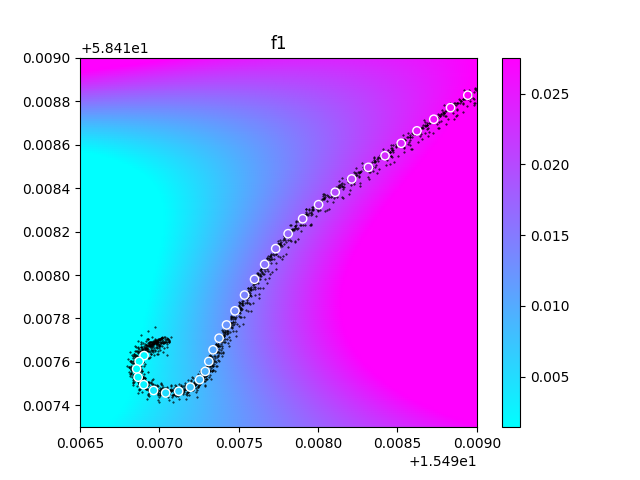
\includegraphics[width=0.775\textwidth]{figures/f1_gp/f1_gp_small_all_data}
    \caption[$f_1$ GP from the first approach]%
    {{\small $f_1$ GP from the first approach.
    The coloured, outlined circles are training data points.
    The black data points are observed \texttt{ObservedPositionEvent}s from all trajectories.
    The regression field is visualised by the gradient background.}}    
    \label{fig:f1-gp-bad}
\end{figure}

\begin{figure}
    \centering
    \begin{subfigure}[b]{0.475\textwidth}
        \centering
        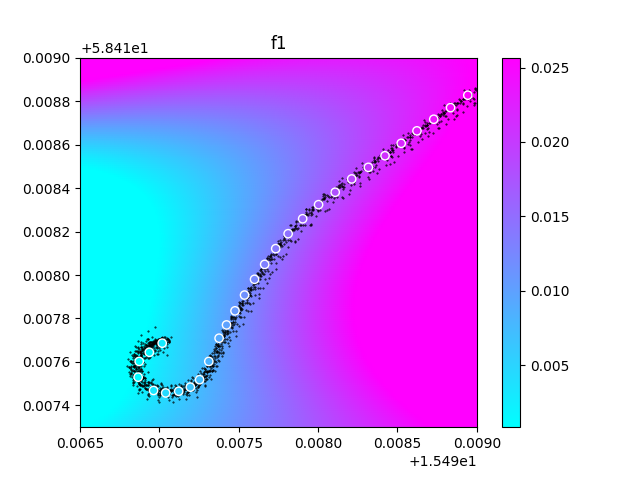
\includegraphics[width=\textwidth]{figures/f1_gp/f1_gp_6e-5_filter}
        \caption[Segment1]%
        {{\small $f_1$ GP trained with a distance filter of $6\times10^{-5}$, which corresponds to around 4 metres.}}    
        \label{fig:f1-gp-1}
    \end{subfigure}
    \hfill
    \begin{subfigure}[b]{0.475\textwidth}  
        \centering 
        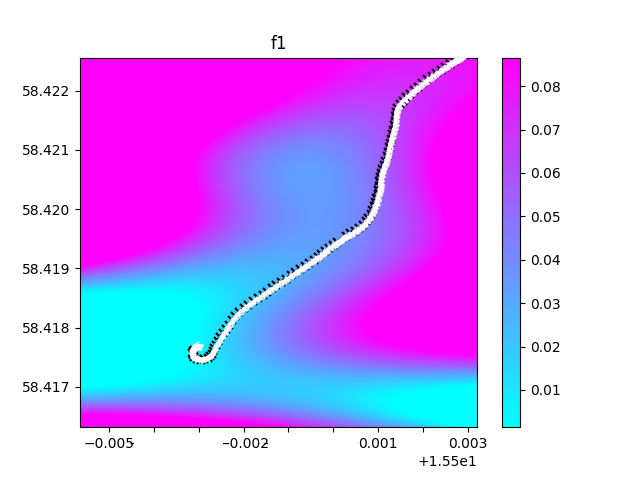
\includegraphics[width=\textwidth]{figures/f1_gp/f1_gp_middle}
        \caption[]%
        {{\small Same $f_1$ GP as in \ref{fig:f1-gp-1}, but visualised on a bigger grid.}}    
        \label{fig:f1-gp-2}
    \end{subfigure}
    \vskip\baselineskip
    \begin{subfigure}[b]{0.475\textwidth}   
        \centering 
        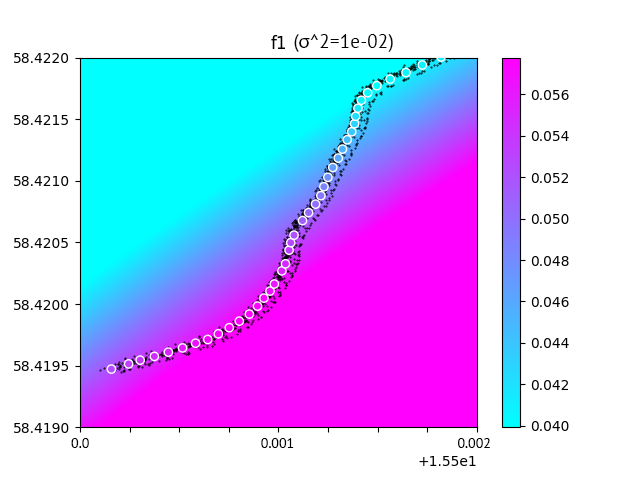
\includegraphics[width=\textwidth]{figures/f1_gp/f1_gp_ARD_1e-2}
        \caption[]%
        {{\small The first segment has been removed from all trajectories.
        Observation noise $\sigma_n^2$ fixed to $10^{-2}$.}}    
        \label{fig:f1-gp-3}
    \end{subfigure}
    \quad
    \begin{subfigure}[b]{0.475\textwidth}   
        \centering 
        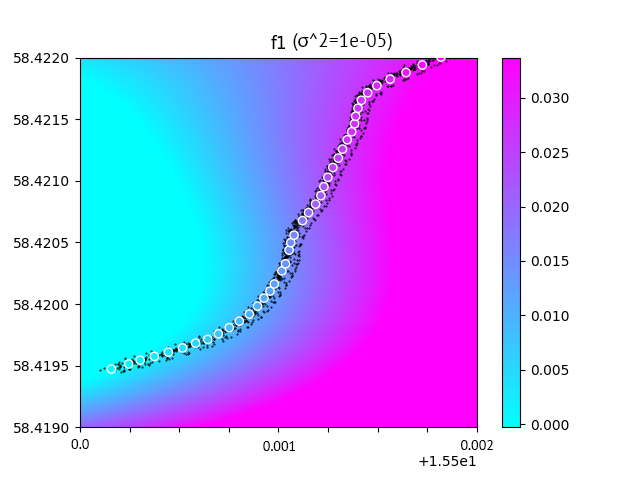
\includegraphics[width=\textwidth]{figures/f1_gp/f1_gp_ARD_1e-5}
        \caption[]%
        {{\small The first segment has been removed from all trajectories. 
        Observation noise $\sigma_n^2$ fixed to $10^{-5}$.}}    
        \label{fig:f1-gp-4}
    \end{subfigure}
    \caption[ $f_1$ GPs from the second approach ]
    {{\small $f_1$ GPs from the second approach. The coloured circles are the training data points.
    The small black points are observed data points from other trajectories.
    The background shows how points are assigned to different $\tau$ values.}} 
    \label{fig:segments}
\end{figure}

The first approach achieved poor results, see Figure \ref{fig:f1-gp-bad}, as points in the beginning of the trajectory are not properly modelled by the $f_1$ GP, since most points had a \textit{Speed} value less than 0.1 m/s.
The coloured, outlined circles are data points used for training the GP.
The black points are \texttt{ObservedPositionEvent}s from trajectories.
The regression field is shown in the gradient background; the colour maps to a $\tau$ value.
The second approach achieves better results.
Figures \ref{fig:f1-gp-1} and \ref{fig:f1-gp-2} show the same model visualised on different grids.
The model does not generalise well, as seen in the larger grid by the blue coloured area in the bottom right corner of \ref{fig:f1-gp-2}.

Figure \ref{fig:f1-gp-3} shows an attempt to improve the general performance of the $f_1$ GP.
The distance filter is the same as in the model shown in \ref{fig:f1-gp-1} and \ref{fig:f1-gp-2}.
However, the first segment has been removed from all trajectories, as the curvature created instabilities in the model.
The effect of the curvature are similar to those which stem from trajectories with self-overlap.
The variance is fixed to $10^{-2}$, which corresponds to a standard deviation of around 6 kilometres in an attempt to prevent overfitting, as many points in the trajectory are close to each other.
This causes the model to overestimate the variance of observations.
Similar results are achieved if the trajectory is downsampled to only use every $n$ data point.
The fixed variance is too large for the model, which causes extremely poor regression.

Figure \ref{fig:f1-gp-4} locks the variance to $10^{-5}$, which corresponds to a few metres in longitude and latitude, similar to the distance filtering.
The specific GPS sensors used in the buses are unknown, but they are in this thesis assumed to have similar precision as GPS-enabled smartphones.
The precision is typically around the range of ca. 5 metres \cite{van2015}.

GP models also typically assume zero mean for the input data, which in this thesis project is achieved by fitting a global re-scaling model to the input data.
The same trajectory used for $f_1$ is used to fit this global re-scaling model.
All trajectory coordinates are centralised and normalised by the global re-scaling model. 
The $f_1$ GPs are trained with a RBF kernel and the hyperparameters are automatically optimised using the GPflow framework.
Automatic Relevance Determination \cite{Rasmussen2006} is used with the RBF kernel to allow for different length-scales in different dimensions.

\section{Segment Self-Overlapping Journeys} \label{sec:segment-self-overlapping-journeys}
After the input space synchronisation, each trajectory if fitted with two GPs.
Journeys are analysed in order to detect self-overlapping, which would cause problems for the GP models, as described in Section \ref{sec:self-overlapping-trajectories}.
Journeys with self-overlap are split at the overlapping points into two segments.
The process recursively analyses each resulting segment and proceeds with splitting the segments as long as self-overlapping is present.
If a journey has multiple segments, each segment is fitted with its own two GPs
\begin{align}
    f_2&: \tau \longmapsto x \\
    f_3&: \tau \longmapsto y
\end{align}
$\tau$ is the relative time of the journey, denoting the progress the bus has made on its journey, $x$ the longitude, and $y$ the latitude.
The $\tau$ values are from the $f_1$ GP, evaluated on the trajectory data.

Once $f_{2_k}$ and $f_{3_k}$ have been trained for each trajectory $k$, the GPs are evaluated on a grid of longitude and latitude points.
The grid is fed to the $f_1$ GP in order to produce a grid of $\tau$ values.
The $\tau$ values are given to the $f_2$ and $f_3$ models and the result is a grid where each point has a longitude and latitude mean and variance, respectively.
The grid is then visualised alongside the observed \texttt{ObservedPositionEvent}s, in order to compare the variance variation.
The $f_2$ and $f_3$ models have a locked data noise $\sigma^2_n$ of $10^{-3}$, which corresponds to a standard deviation of around 1500 metres, separate from the data noise used in GP $f_1$.

\section{Probability Models} \label{sec:probability-models}
The GPs $f_2$ and $f_3$ each describe the mean ($\mu_x$ and $\mu_y$, respectively) and variance ($\sigma_x^2$ and $\sigma_y^2$, respectively) at each point in the fitted segment or journey.
The probability for various coordinate pairs $p((x_\star,y_\star))$ is of interest in this thesis project, which can be calculated with two different approaches.

\subsection{Mixture of Gaussian Process Model with Uniform Prior}
The first approach is to see all of the trajectory models for the same bus line as a Mixture of Gaussian Process (MoGP) model.
An observed $(x_\star, y_\star)$ coordinate is thus assumed to be generated from one of the GP models in the MoGP.
The prior on the MoGP model is assumed to be uniform.
The probability of $(x_\star, y_\star)$ for each trajectory model $k$ is 
\(
    p_k((x_\star,y_\star)) = \mathcal{N}((x_\star,y_\star); \mu_k, \Sigma_k)
\), where
\begin{align}
\mu_k &= \begin{bmatrix} \mu_{k_x} \\ \mu_{k_y} \end{bmatrix} \\
\Sigma_k &= \begin{bmatrix} \sigma^2_{k_x} & 0 \\ 0 & \sigma^2_{k_y} \end{bmatrix}
\end{align}
is the mean and covariance of the point evaluated at $(x_\star,y_\star)$.
In the covariance matrix $\Sigma_k$, longitude and latitude is assumed to be independent.
As the MoGP prior is uniform, the probability of $(x_\star, y_\star)$ is given by
\begin{equation}
    p((x_\star, y_\star)) = \frac{1}{K}\sum_{k=1}^K p_k((x_\star,y_\star)),
\end{equation}
where $K$ is the number of trajectory models.

\subsection{Unimodal Mixture of Gaussian Process Model by Combining}
In order to make a unimodal approximation of the MoGP model, $f_{2_k}$ and $f_{3_k}$ are point-wise combined for each trajectory $k$.
However, it is not an approximation with respect to assumptions made in this thesis project.
The assumption is that the observed trajectories are drawn from a single unimodal distribution over functions with Gaussian noise with varying variance.
The aggregation is done by using the Combining equations \ref{eq:combining-mean} and \ref{eq:combining-var} from Section \ref{sec:trajectory-aggregation}.
The Combining approach is preferred over the Fusion approach in this particular problem, as the model is trying to capture the variation of GPS positions.
It is thus beneficial to use an aggregation approach which tries to capture and aggregate the variance of each local trajectory model.
They are applied as follows (with the notation changed to represent the notation used in this chapter):
\begin{align}
    \mu_x(x^*) &= \frac{\sum_{k=1}^{K} M_k\mu_{k_x}(x^*)}{\sum_{k=1}^{K} M_k}, \label{eq:combined-mu-x} \\
    \mu_y(y^*) &= \frac{\sum_{k=1}^{K} M_k\mu_{k_y}(y^*)}{\sum_{k=1}^{K} M_k}, \label{eq:combined-mu-y} \\
    \sigma_x^2(x^*) &= \frac{\sum_{k=1}^{K} M_k\Big(\sigma_{k_x}^2(x^*) + \mu_{k_x}^2(x^*)\Big)}{\sum_{k=1}^{K} M_k} - \mu_x(x^*)^2, \label{eq:combined-var-x} \\
    \sigma_y^2(y^*) &= \frac{\sum_{k=1}^{K} M_k\Big(\sigma_{k_y}^2(y^*) + \mu_{k_y}^2(y^*)\Big)}{\sum_{k=1}^{K} M_k} - \mu_y(y^*)^2, \label{eq:combined-var-y}
\end{align}
where
\begin{itemize}
    \item $M_k$ is the number of trajectories used to train $f_{2_k}$ and $f_{3_k}$.
    In this thesis project, each trajectory $k$ is trained on its own $f_{2_k}$ and $f_{3_k}$ $\Rightarrow$ $M_k = 1$ for all $k = 1,\dotso,K$ trajectories.
    \item $x^*$ and $y^*$ are index slices (points) to evaluate the MoGP model at.
    \item $\mu_{k_x}$ and $\mu_{k_y}$ is the predicted mean of the evaluated point at the index slice of x (longitude) and y (latitude), respectively. 
    \item $\sigma_{k_x}^2$ and $\sigma_{k_y}^2$ is the predicted variance of the evaluated point at the index slice. 
\end{itemize}

Equations \ref{eq:combined-mu-x}-\ref{eq:combined-var-y} can thus be simplified to
\begin{align}
    \mu_x(x^*) &= \frac{\sum_{k=1}^{K} \mu_{k_x}(x^*)}{K} \label{eq:simplified-combined-mu-x} \\
    \mu_y(y^*) &= \frac{\sum_{k=1}^{K} \mu_{k_y}(y^*)}{K} \label{eq:simplified-combined-mu-y} \\
    \sigma_x^2(x^*) &= \frac{\sum_{k=1}^{K} \Big(\sigma_{k_x}^2(x^*) + \mu_{k_x}^2(x^*)\Big)}{K} - \mu_x(x^*)^2 \label{eq:simplified-combined-var-x} \\
    \sigma_y^2(y^*) &= \frac{\sum_{k=1}^{K} \Big(\sigma_{k_y}^2(y^*) + \mu_{k_y}^2(y^*)\Big)}{K} - \mu_y(y^*)^2 \label{eq:simplified-combined-var-y}
\end{align}

The equations \ref{eq:simplified-combined-mu-x}-\ref{eq:simplified-combined-var-y} give the combined unimodal MoGP model at index slice $(x^*, y^*)$
\begin{align}
\mu((x^*, y^*)) &= \begin{bmatrix} \mu_x(x^*) \\ \mu_y(y^*) \end{bmatrix} \\
\Sigma((x^*, y^*)) &= \begin{bmatrix} \sigma^2_x(x^*) & 0 \\ 0 & \sigma^2_y(y^*) \end{bmatrix}
\end{align}
which gives the probability of an arbitrary point $(x_\star, y_\star)$: $p(x_\star, y_\star) = \mathcal{N}((x_\star, y_\star); \mu, \Sigma)$

\section{GPS Variance Estimation Results} \label{sec:gps-var-result}

The MoGP model is visualised by evaluating the model on a grid of longitude and latitude values.
The results from the MoGP model with uniform prior is visualised in Figure \ref{fig:gps-mixture} for three segments of a bus line.
The grid is fed to the $f_1$ GP and thus converted into a grid of $\tau$ values.
The $\tau$ values are given to the $f_2$ and $f_3$ GPs, which returns the predicted longitude and latitude mean and variance, respectively. 
The predicted means and variances are used to create Gaussian distributions for each longitude and latitude pair in the grid.
The probability density function (PDF) is calculated for each Gaussian distribution and divided by the number of GPs in the MoGP model.

The unimodal MoGP model is visualised by evaluating the MoGP model on a grid of longitude and latitude values.
The same approach as in the MoGP model with uniform prior is used.
The $f_2$ and $f_3$ GPs are combined using the Combining formula.
The PDF is calculated for the combined model and is integrated with the grid resolution in order to create a probability distribution.
Figure \ref{fig:gps-variation-estimation} shows the GPS variation for three segments of a bus line.
The results are similar to the MoGP model with uniform prior.

\begin{figure}
    \centering
    \begin{subfigure}[b]{0.475\textwidth}
        \centering
        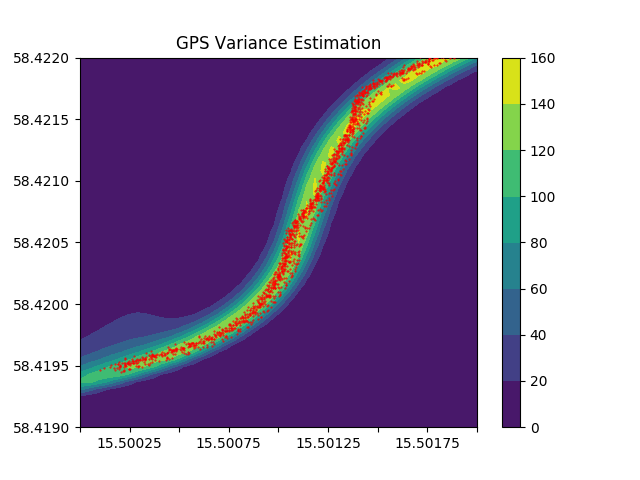
\includegraphics[width=\textwidth]{figures/gps_var/f1_ard_contour_segment1_pdf_all}
        \caption[]%
        {{\small Segment 1 - Beginning of bus line.}}    
        \label{fig:contour-segment-1-mixture}
    \end{subfigure}
    \hfill
    \begin{subfigure}[b]{0.475\textwidth}  
        \centering 
        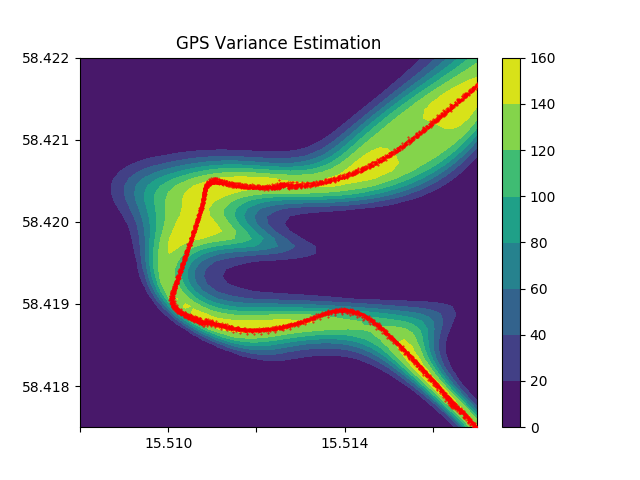
\includegraphics[width=\textwidth]{figures/gps_var/f1_ard_contour_segment2_pdf_all}
        \caption[]%
        {{\small Segment 2 - Middle of the bus line.}}    
        \label{fig:contour-segment-2-mixture}
    \end{subfigure}
    \vskip\baselineskip
    \begin{subfigure}[b]{0.475\textwidth}   
        \centering
        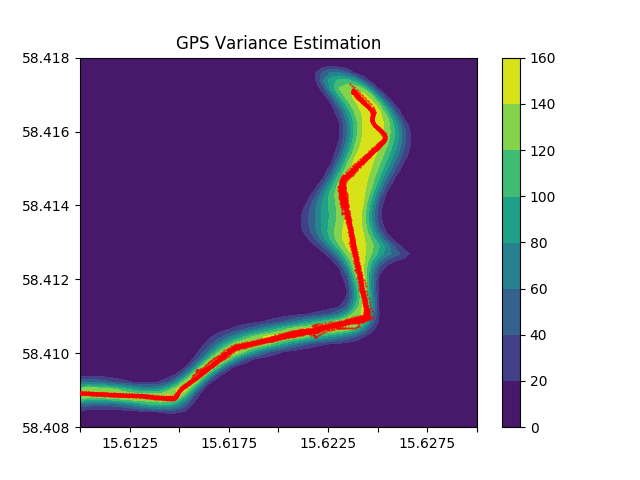
\includegraphics[width=\textwidth]{figures/gps_var/f1_ard_contour_segment3_pdf_all}
        \caption[]%
        {{\small Segment 3 - End of the bus line.}}    
        \label{fig:contour-segment-3-mixture}
    \end{subfigure}
    \caption[ GPS variance variation estimation for the MoGP model ]
    {{\small GPS variance variation estimation for the MoGP model.
    Shows the PDF of GPS positions for a given bus line.
    The model uses a fixed data noise of $10^{-3}$.
    The red dots are \texttt{ObservedPositionEvent}s from the data set.
    The Y-axis is the latitude coordinates and the X-axis is the longitude coordinates.}} 
    \label{fig:gps-mixture}
\end{figure}

\begin{figure}
    \centering
    \begin{subfigure}[b]{0.475\textwidth}
        \centering
        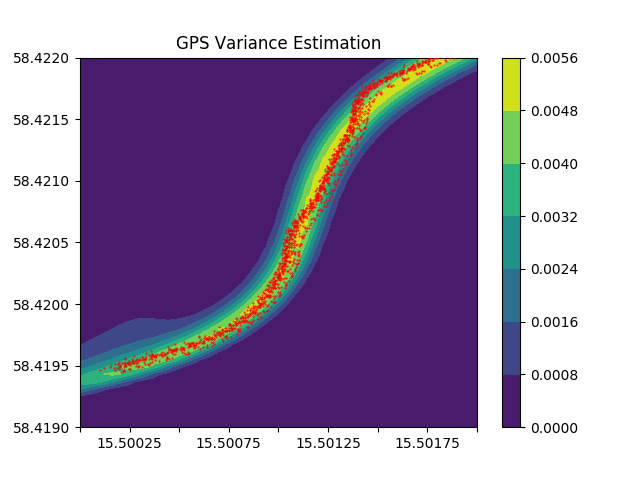
\includegraphics[width=\textwidth]{figures/gps_var/f1_ard_contour_segment1_combine}
        \caption[]%
        {{\small Segment 1 - Beginning of bus line.}}    
        \label{fig:contour-segment-1}
    \end{subfigure}
    \hfill
    \begin{subfigure}[b]{0.475\textwidth}  
        \centering 
        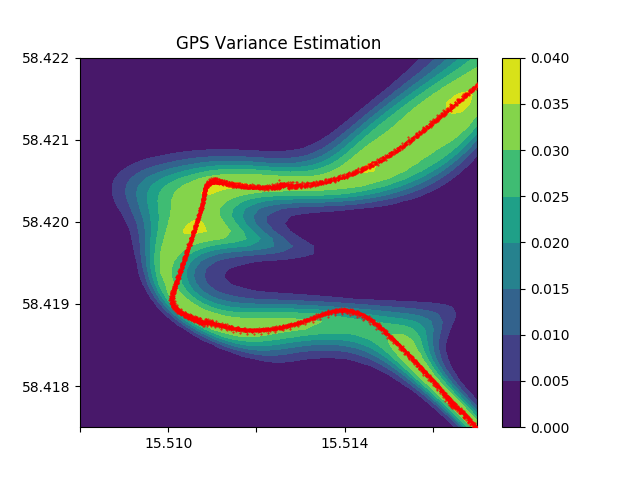
\includegraphics[width=\textwidth]{figures/gps_var/f1_ard_contour_segment2_combine}
        \caption[]%
        {{\small Segment 2 - Middle of the bus line.}}    
        \label{fig:contour-segment-2}
    \end{subfigure}
    \vskip\baselineskip
    \begin{subfigure}[b]{0.475\textwidth}   
        \centering
        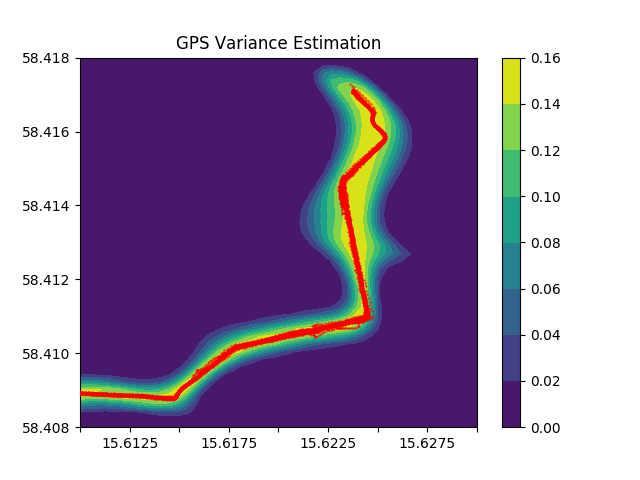
\includegraphics[width=\textwidth]{figures/gps_var/f1_ard_contour_segment3_combine}
        \caption[]%
        {{\small Segment 3 - End of the bus line.}}    
        \label{fig:contour-segment-3}
    \end{subfigure}
    \caption[ GPS variance variation estimation for the unimodal model ]
    {{\small GPS variance variation estimation for the unimodal model.
    Shows the probability that a GPS position is observed for a given bus line.
    The model uses a fixed data noise of $10^{-3}$.
    The red dots are \texttt{ObservedPositionEvent}s from the data set.
    The Y-axis is the latitude coordinates and the X-axis is the longitude coordinates.}} 
    \label{fig:gps-variation-estimation}
\end{figure}

\section{Discussion} \label{sec:gps-var-discussion}

The ridges of the combined probability distributions presented in Figure \ref{fig:gps-variation-estimation} all follow the observed data points well.
However, the probability of observing certain GPS positions are low, even at the ridge of the probability distribution, which is surrounded by the observed data points.
This is probably due to a few things:
    \begin{enumerate}
        \item Though the $f_1$ GP is improved compared to the first approach, it is still not perfect and generalises poorly.
        It creates large areas of uncertainty, where similar values are mapped to the same $\tau$ value.
        This affects the training of the $f_2$ and $f_3$ GPs, as the data is dependent on the transformation (synchronisation) from $f_1$.

        \item Individual longitude or latitude coordinates close to a cluster of observed positions achieve a probability of ca. 0.8-0.9.
        However, it is generally the case that if the probability of a longitude coordinate is high, then the probability of the latitude coordinate for that grid point is low.
        As the longitude and latitude coordinates are assumed independent, the probability for a grid point is $p(lat_{point}) * p(lng_{point})$, where one is close to 1 and the other one small (< 0.1).
        This is partially solved if the PDF is integrated on a larger interval, as more of the probability density is captured in one point.
    \end{enumerate}

The variance variation is larger at certain locations on the bus line.
In the end segment shown in Figure \ref{fig:contour-segment-3}, this occurs in an environment surrounded by tall buildings.
This might be a reason for the increased variation, though it is not adequately reflected in the observed training data.
A more likely reason for the increased variance in the figure is due to a poor $f_1$, $f_2$, and $f_3$ models unable to handle the sharp trajectory turns.  
The $f_1$ GP might perform better if it is trained on segments of the trajectory, instead of trying to learn the full trajectory.
The removal of the first segment from all trajectories is a necessary step in order to improve the generalisation of the $f_1$ GP.
However, as discussed above, it might not have been enough in order to create a generally robust model.

\subsection{Evaluation and Assumptions}
In this thesis project, the variance variation is evaluated visually.
Ideally, other metrics would be applied, such as determining locations where the variation is the smallest and the biggest.
These metrics could be useful when looking at the impact of the surrounding environment on the GPS variance.
The kernels used are evaluated both visually and by looking at the resulting hyperparameters after the optimisation step.
If the likelihood of the data is optimised to be small ($10^{-6}$), it could be a result of overfitting to the linear trend of the data.

The evaluated data is assumed to have an inherent noise of $10^{-5}$, which is the measured accuracy of GPS-enabled smartphones.
The noise specified for the $f_2$ and $f_3$ GPs are fixed to $10^{-3}$.
They are tested with a data noise of $10^{-5}$, as in the case of $f_1$, but this resulted in barely any visible variation.
The variation shown in Figure \ref{fig:gps-variation-estimation} is thus dependent on the fixed noise of the observed data.
This parameter needs further investigating, as the current choice results in perhaps larger variation than expected.

\subsection{Model Optimisation}
The models in this thesis project are optimised using the L-BFGS-B algorithm implemented in open-source software Scipy\footnote{https://docs.scipy.org/doc/scipy/reference/index.html}.
It would perhaps have been better to estimate the hyperparameters through Markov chain Monte Carlo (MCMC) using Hamiltonian Monte Carlo (HMC) sampling, implemented in the GPflow framework.
The use of sampling to estimate hyperparameters, and further optimise them with the maximum a posteriori (MAP) of the sampled posterior as initial value would definitely be useful to investigate in future work.

\subsection{Trajectories}
Due to limited time and limited processing power, the number of trajectories used for the models is restricted to 37.
The trajectories are all collected from the same day.
It took, on average, eight hours to retrain all the models, which caused changes to be expensive time-wise.
It is not always immediately clear if a change generalises well or not.
For example, some configurations show extremely poor results on only a small number of trajectories, while the results are average on the others.
The training time proved to be a huge drain on the effectivity of the feature extraction and model optimisation.

The aim of the thesis project is to use trajectories from multiple days in order to determine an eventual bias of the positions depending on day and time.
This thesis project creates a foundation where this analysis is possible in a future work.   

Only trajectories from buses are analysed in this thesis project.
It would have been interesting to see how the data from trains differed and how their variance variation compared to the variation from the buses.

\section{Future Work}
There are a few aspects which could be improved in future work.
The improvement of the $f_1$ GP would be a main priority, given more time to the thesis project.
The $f_1$ GP is the backbone of the $f_2$ and $f_3$ models trained for the GPS variance variation estimation.
The idea of splitting a trajectory into smaller segments and train one $f_1$ GP for each segment is sound.

\subsection{Variation Over Multiple Days}
Future improvements of the GPS variation estimation would be to train the models on data from different days, using the day and time of the day as a feature.
This would allow for the analysis of how the GPS variation changes throughout a day and over a span of days.
The use of a periodic kernel would perhaps also be useful, in order to capture the periodicity of satellites.
Improvements made to the dataset could further benefit this analysis.
For example, information about the number of satellites used, which satellites are available, and their respective positions, would give information about the potential periodicity of the variation.

\begin{figure}[ht!]
    \centering
    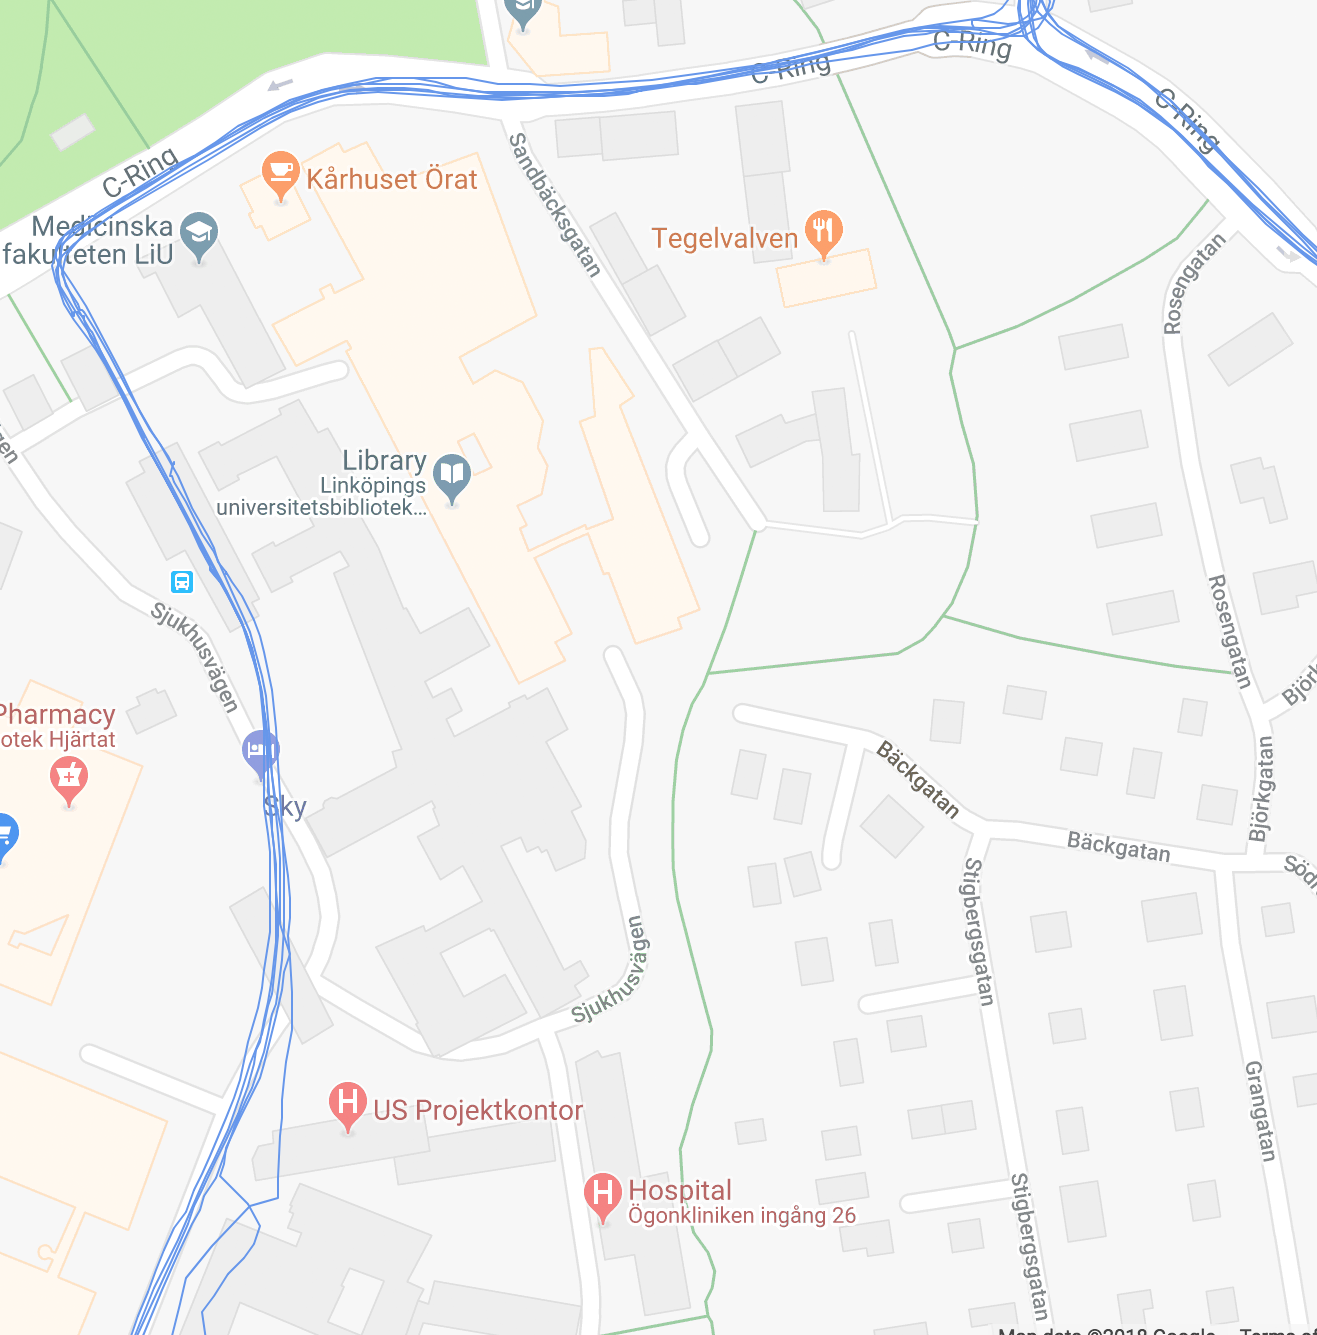
\includegraphics[width=0.7\textwidth]{figures/gps_map_problem}
    \caption[Real-world example of multiple buses driving on a road not correctly modelled by Google Maps]
    {\small Real-world example of multiple buses driving on a road not correctly modelled by Google Maps.
    For example, at "Sjukhusvägen" the buses are driving through a building according to Google Maps.
    In this particular scenario the area has received major road re-structuring and renovation.
    The Google Maps representation is thus likely outdated.}
    \label{fig:gps-map-problem}
\end{figure}

\subsection{Road Segments}
Another area not investigated in this thesis project is the use of the Google Maps Roads API\footnote{https://developers.google.com/maps/documentation/roads/intro}.
The API maps GPS coordinates to the closest geographical road segment.
The road segments could, for example, in future work be used as a "truth" when determining the variation of GPS signals.
However, manual inspection of journeys done in the pre-processing step highlights scenarios with discrepancies between roads in Google Maps and actual roads the buses travelled.
The Google Maps roads are in these scenarios usually incorrectly drawn or has missing roads.
Figure \ref{fig:gps-map-problem} shows such a real-world example.
The discrepancies would cause problems if used naïvely together with the Google Maps Roads API.
These journeys would have to be detected and either handled or ignored.
The detection could be done by looking at the distances to the closest Google Maps Roads segments.
The distances would be roughly similar for all the journeys, as in Figure \ref{fig:gps-map-problem}.
Since the distances would be roughly similar they could be averaged and interpreted as a bias to the roads.
Applying the bias-interpretation methodology would result in a more generalised model using the Google Maps Roads API.
Ignoring the journeys with discrepancies could also be seen as feasible, given that the occurrence is rare.
Before using the simpler approach of ignoring journeys with discrepancies, a deeper analysis needs to be conducted.
